% !TeX root = ../../../../thesis.tex

\subsection{AC}
\label{subsec:ac-evaluation}


The AC testbed has three commercial LEDs, as explained in \autoref{subsec:ac-testbed}.
Therefore three IDs will be for the LEDs with a fourth ID being used to represent an LED in an off state.
From \autoref{tbl:correlation-gold-families}, we can see that for $m = 3$, the number of simultaneous transmitters such that no destructive interference takes place, requires a code length of 127 or higher.
With the AC testbed, the experiments were performed with a constant modulation frequency of 10 kHz.
%Two successive samples are $\frac{1}{10000} = 0.1$ ms apart, except for when the triggering circuit detects that no modulation or sampling can take place anymore.
%In that case the sampling and modulation is paused until the triggering circuit detects that modulation and sampling can take place again.


In \autoref{fig:raw-ac-testbed-adc-data} the incoming signals to the current sampler can be seen.
The raw data from the ADC can be seen as well as the output of the triggering circuit.
From 2.5 ms until 6 ms in the figure, the charging peaks of the capacitor can be seen as explained in \autoref{subsec:ac-modulator}.
In the same time window, the output of the triggering circuit can also be seen.
The triggering output is used to filter out the charging peaks and only the aggregated IDs are left.
The aggregated IDs can be seen in the time window from 6 ms until 14 ms.
This is the window which holds the encoded data and that data is retrieved by using the triggering circuit to detect when to start and stop looking for the encoded data.

\begin{figure}[ht]
  \centering
  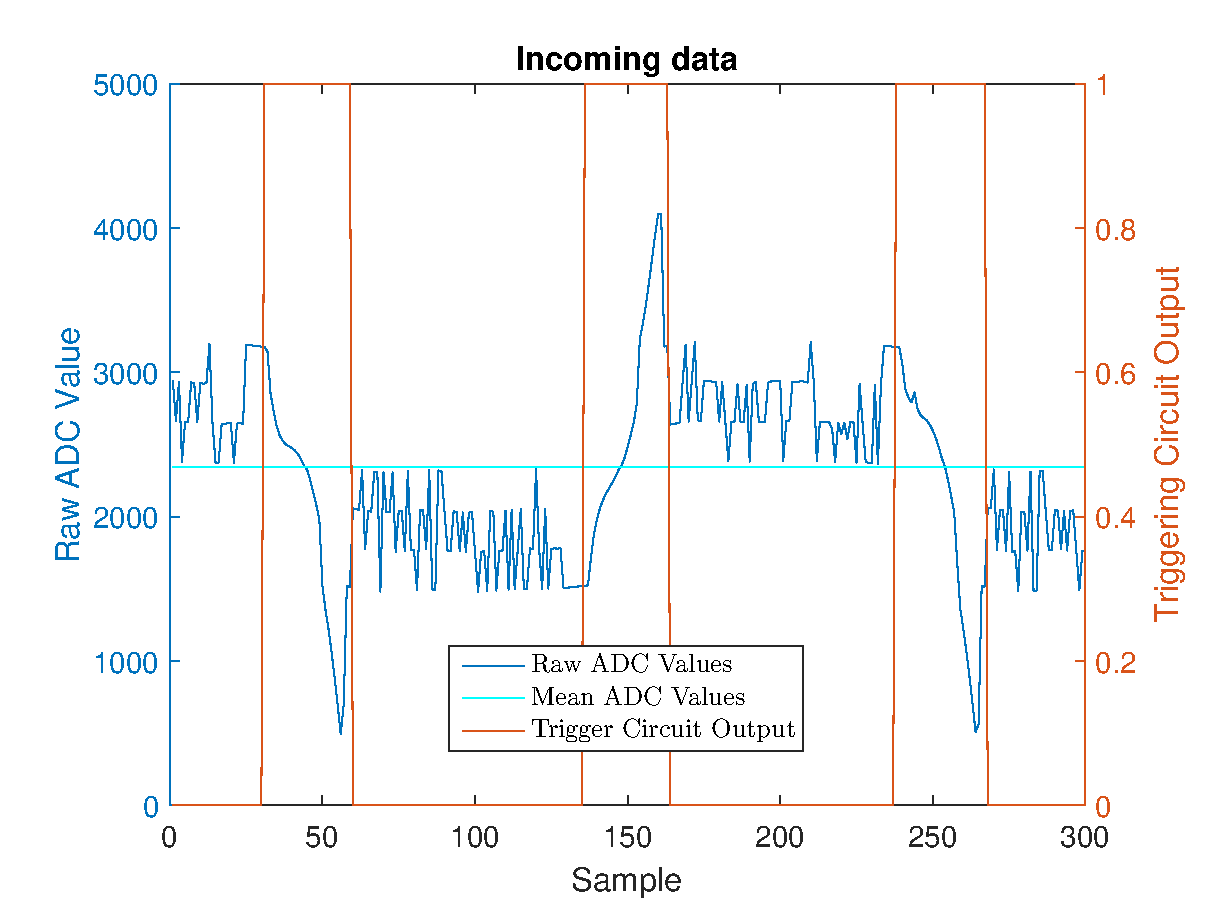
\includegraphics[width=0.8\textwidth]{chapters/evaluation-chapters/hardware/ac/raw-ac-testbed-adc-data.eps}
  \caption{Incoming data to the AC current sampler. The raw ADC values are plotted as well as the triggering circuit output. Gold sequence of length 127.}
  \label{fig:raw-ac-testbed-adc-data}
\end{figure}

As is the case in an AC environment, the current that will flow is both positive and negative.
As explained in \autoref{subsec:ac-current-sampler} to overcome this bipolarity problem the voltage measured over the series resistor is added with a constant reference voltage in order for the ADC to only measure positive voltages.
The encoded data that is shown in \autoref{fig:raw-ac-testbed-adc-data} is now filtered out with help of the triggering circuit.
The next step is to subtract the reference voltage from each sample of the encoded data.
And then the absolute value of the result is considered.
The result of the processing of the raw ADC data can be seen in \autoref{fig:processed-ac-testbed-adc-data}.
In this figure the ADC values are on the left y-axis and the current on the right y-axis.

\begin{figure}[ht]
  \centering
  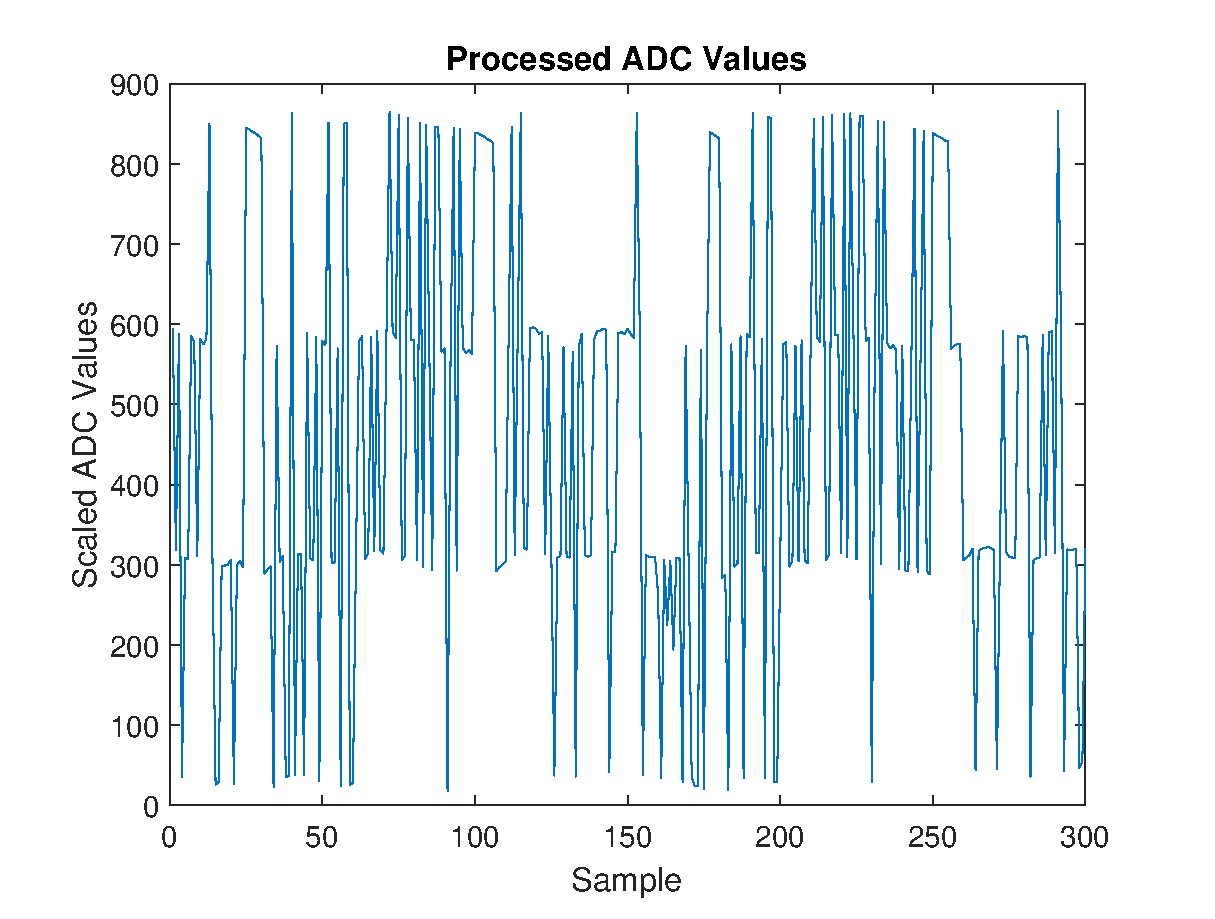
\includegraphics[width=0.8\textwidth]{chapters/evaluation-chapters/hardware/ac/processed-ac-testbed-adc-data.eps}
    \caption{Fully processed ADC values, where four distinguishable levels can be seen. With the on-state from zero to all three LEDs, on the AC testbed.}
  \label{fig:processed-ac-testbed-adc-data}
\end{figure}

In \autoref{fig:processed-ac-testbed-adc-data}, four distinguishable current levels can be seen.
%Just like in the DC evaluation, these distinct current levels come from the IDs that the LEDs are encoding.
When all the LEDs are encoding a `0', the current is (almost) zero, when one LED is encoding a `1' the current is approximately 100 mA and so on.
With this processed signal the correlation calculations can be done to identify which LEDs are on and which are off.


%To avoid confusion about the x-axis of \autoref{fig:raw-ac-testbed-adc-data} and \autoref{fig:processed-ac-testbed-adc-data}: The amount of time in both figures is the same, however parts of the raw data of \autoref{fig:raw-ac-testbed-adc-data} are filtered out so why would the time still be the same.
%The time is the same for both figures, because in the processed data which is shown \autoref{fig:processed-ac-testbed-adc-data} was created with the original raw ADC signal.
%And the original raw signal was much longer than the 30 ms shown in this report.
%This means that the amount of encoded data in \autoref{fig:processed-ac-testbed-adc-data} is more than what is shown in \autoref{fig:raw-ac-testbed-adc-data}.


Now that the raw ADC signal is processed, the correlation can be calculated.
In \autoref{fig:correlation-ac-testbed}, two signals and one line are plotted.
The straight line represents the threshold, which is based on the length of the codes used, see \autoref{sec:interference-solution}.
The other two signals represent the outcome of the correlation with the ID of two LEDs.
One of those IDs is from an LED which is on and the other ID is from the LED which represents an LED in an off state.
The correlation results from the LED which is in an off state, stay below the threshold for all points in time.
This is a good result, since being below the threshold line means that the corresponding LED is off, which in this case is actually true.

The other correlation result, shown in \autoref{fig:correlation-ac-testbed} comes from the ID which corresponds to an LED which is on and modulating.
The results of this correlation show two noticeable peaks above the threshold.
These peaks indicate that the ID is present in the sampled current signal by the smart-meter.
There are two peaks, because the LED is continuously transmitting its ID and the length of the ID in combination with the modulation frequency can be transmitted two times in the 30 ms window.
All the peaks mean the same thing: The ID is present in the sampled current signal.
Since this ID represents an LED which is on, these peaks are correct results.% as they indicate that the LED is indeed on.

The evaluation as discussed above for the AC testbed has been run in a similar fashion compared to the DC testbed evaluation.
The evaluation was run for more than ten times.
And for each run the duration was approximately five minutes.
Each run showed the same results as presented in \autoref{fig:correlation-ac-testbed}.
All the results we obtained, were correct.
This means that there are only true-positives and true-negatives.
So the precision, recall and the F-measure are all equal to $1$.% according to \autoref{eq:precision}, \autoref{eq:recall} and \autoref{eq:F-measure}, respectively.

\begin{figure}[t]
	\centering
	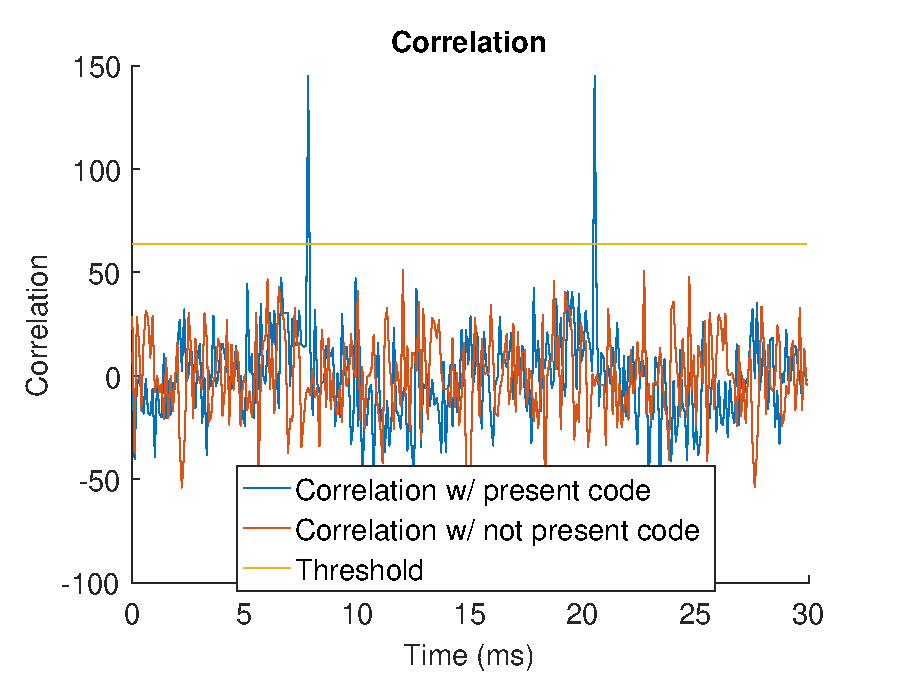
\includegraphics[angle=0,width=\textwidth,keepaspectratio]{chapters/evaluation-chapters/hardware/ac/correlation-ac-testbed.eps}
	\caption{Correlations results from the IDs to identify which LEDs are on and off, with the decision threshold. With a sequence length of 127 on the AC testbed.}
	\label{fig:correlation-ac-testbed}
\end{figure}

